%% A 3-page report describing the central aspects of your A* program, such as
% the agenda and how it is managed. This must clearly and concisely document
% the generality of your program: it should illustrate how your program can
% easily be reused on other search tasks, with only a little subclassing needed
%for each new task. So the core code should NOT have details specific to the
% navigation task. The report must also describe your heuristic function and
% your method for generating successor states. The report must NOT exceed 3
% pages, including all diagrams, code segments, etc. (4 points)
\section{Central aspects of the A* program}
This report describes our implementation of the A* algorithm and our solution to the navigation problem.

\subsection{The agenda and how it is managed}

Three search routines had to be supported out of the same base algorithm with a flick of a notch. This is quite easy when you know that substituting the heap with either a queue or a stack, you get respectively a breadth-first- and a depth-first-algorithm that is suitable to solve the same problems, though with different performance and optimality measures.

Substituting the heap is done easily in python, and you can then define some common pop and push methods that modify the agenda, whether its a heap, stack or a queue (see figure \ref{code:manage_agenda}). In the code snippet, `opened` is the datastructure of your choice.

\lstinputlisting[emph={open_push,open_pop,OPEN,A_STAR,BFS,DFS},label={code:manage_agenda},caption={Management of the agenda.}]{module_1/code_snippets/manage_agenda.py}

\subsection{Generality of the program}

\begin{figure}[h!]
	\centering
	\resizebox {!} {8cm} {
		\begin{tikzpicture} 
			\umlclass{BestFirstSearch}{
				start : SearchState
			}{
				+ attach\_and\_eval(child : SearchState, parent : SearchState) : void \\
				+ propagate\_path\_improvements(parent : SearchState) : void \\
				+ best\_first\_search() : SearchState \\
				+ \umlvirt{arc\_cost(a : SearchState, b : SearchState) : double} \\
				+ \umlvirt{create\_root\_node() : SearchState} \\
				+ open\_push(opened : [], node : SearchState) : void \\
				+ open\_pop(opened : []) : SearchState \\
				+ node\_closed(node : SearchState, t\_0 : long, generated : {}, opened : [], closed : []) : void
			}
			\umlclass[right=13cm of BestFirstSearch.north, anchor=north]{SearchState}{
				state : object \\
				sid : string \\
				status : int \\
				parent : SearchState \\
				kids : [] \\
				g : double \\
				h : double \\
				f : double
			}{
				+ add\_child(child : SearchState) : void \\
				+ \umlvirt{create\_state\_identifier() : string} \\
				+ \umlvirt{heuristic\_evaluation() : double} \\
				+ \umlvirt{is\_solution() : boolean} \\
				+ \umlvirt{solution\_length() : double} \\
				+ \umlvirt{generate\_all\_successors() : SearchState}
			}
			\umlclass[below=8cm of SearchState.north, anchor=north]{NavigationState}{
				visited : [] \\
				current\_pos : []
			}{
				+ create\_state\_identifier() : string \\
				+ heuristic\_evaluation() : double \\
				+ is\_solution() : boolean \\
				+ solution\_length() : double \\
				+ generate\_all\_successors() : SearchState \\
				+ euclidean\_distance(a : [], b : []) : double \\
				+ manhattan\_distance(a : [], b : []) : double \\
				+ print\_level() : void
			}
			\umlclass[below=6cm of BestFirstSearch.north, anchor=north]{NavigationBfs}{}{
				+ arc\_cost(a : SearchState, b : SearchState) : double \\
				+ create\_root\_node() : SearchState
			}
			\umlinherit[geometry=-|, anchors=north and south]{NavigationState}{SearchState}
			\umlinherit[geometry=-|, anchors=north and south]{NavigationBfs}{BestFirstSearch}
			\umlunicompo[geometry=-|, stereo=start, anchors=east and 164, pos stereo=0.5]{BestFirstSearch}{SearchState}
		\end{tikzpicture}
	}
	\caption{Class diagram for the navigation task.}
\end{figure}

Figure \ref{run:examples} shows the class diagram for the navigation problem. As seen, each new problem needs to define two classes that inherit from `search\_state' and `best\_first\_search', respectively. Two methods, `create\_root\_node' and `arc\_cost', has to be overidden in the subclass of `best\_first\_search' for it to work. Likewise, the subclass of `search\_state' has to implement `heuristic\_evaluation', `create\_state\_identifier', `generate\_all\_successors', `is\_solution' and `solution\_length'. Most of these methods can be reused in similar problems, and this makes almost no effort to have a new type of problem solver up and running in no time.

To ensure generality we started by implementing the basic checkers example in
the \emph{Essentials of A*} document, and then implemented the navigation specialization
of the exercise. Having two implementations in Module 1 forced us to keep the
structure outlined in the document throughout our optimization attempts.

\subsection{Heuristics}
Both the \emph{Manhattan distance} and \emph{Euclidean distance} has been tested on the navigation problem. Each adjusted the behaviour of the agent. Using the manhattan distance the agent seems to prefer minimizing the amount of \(90 deg\) turns before reaching the final goal. The euclidean distance seems to do the quite opposite, and the agent goes straight towards the target even though the agent cannot move diagonally. It tries to emulate the behaviour of walking diagonally and follows a diagonal line between the current position and the goal. In the example board number two (Figure \ref{run:examples}), the manhattan distance wins by generating least amount of nodes, because it moves right and then up without encounter an obstacle. 

The euclidean agent has to avoid an obstacle and therefore is generating a few more nodes. On the other hand, in example 5 (Figure \ref{run:examples}), the euclidean agent slips through the opening between the two last obstacles, while the manhattan agent needs to explore the area before the right-most obstacle. The performance of the agent depends on the heuristics and arc-cost compared with the structure of the board. Switching the euclidean and manhattan when using diagonal moves, seem to result in similar end results, though either of the two may visit more states than the other.

The arc-cost has to be changed whether the agent can move diagonal or not. A arc-cost below 1 is suitable for strict axis-movements and a arc-cost above 1 for diagonal movement. If the arc-cost is below 1 for diagonal movement, the agent would do unnecessary and dramatic turns which result in wierd behavior.

\begin{figure}[h!]
	\centering
	\begin{minipage}{\textwidth}
		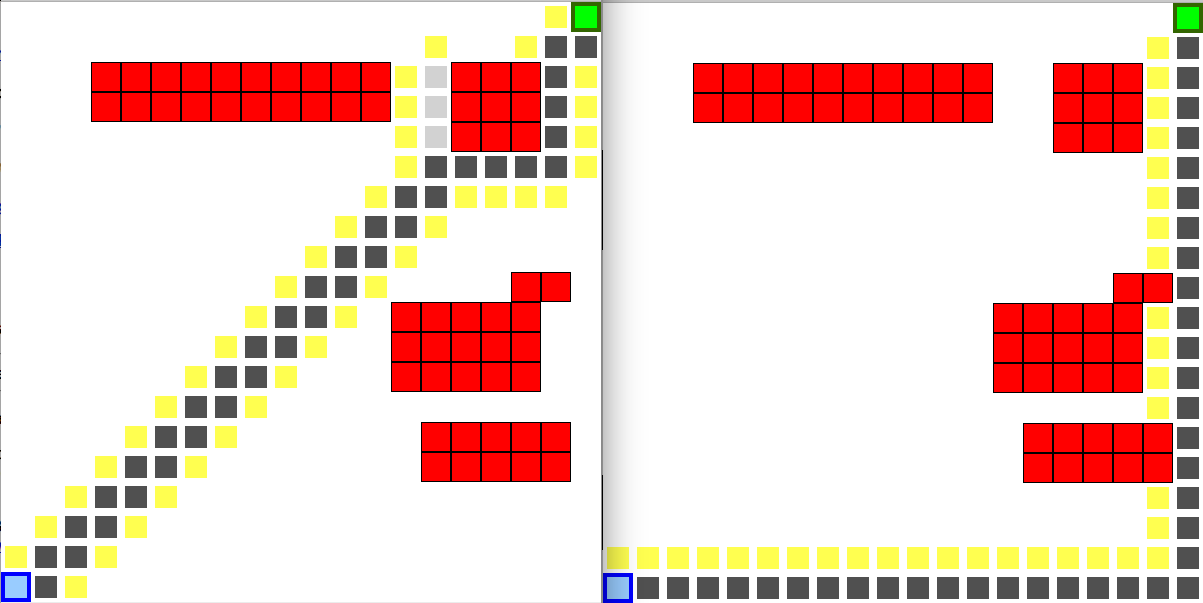
\includegraphics[width=0.5\textwidth]{module_1/images/run_ex2}
		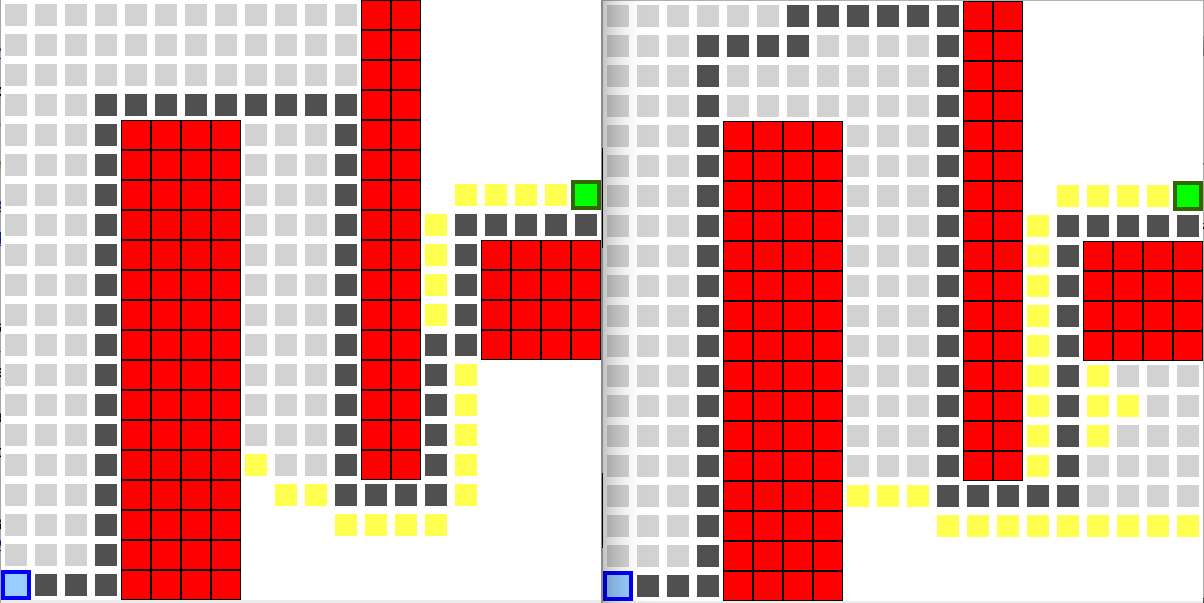
\includegraphics[width=0.5\textwidth]{module_1/images/run_ex5}
	\end{minipage}
	\caption{Comparing euclidian distance and manhattan distance in board example 2 and 5, respectively.}
	\label{run:examples}
\end{figure}

\subsection{Generating successor states}
From each viable state, a maximum of eight possible successor states can be created, each by moving in each direction from its currently held position; NORTH, SOUTH, EAST, WEST, NORTH-EAST, NORTH-WEST, SOUTH-EAST, SOUTH-WEST. If the diagonal variable is set, eight states are generated, else only four is generated, as seen in figure \ref{code:succesor-generation}.

Other considered limitations are that the new position should be inside the given dimensions of the board, and that obstacles are not walkable, together with unnecessity to visit positions that previously have been visited. Every state that is within the scope of those limitations, is created and added to the heap. 

\lstinputlisting[label={code:succesor-generation},caption={Successor generator vectors.}]{module_1/code_snippets/gen_successors.py}

\subsection{Runs on the provided boards}
Table \ref{table:results} summarize the results of a run on each of the provided problems.
\begin{table}[h]
	\centering
	\begin{minipage}{\textwidth}

		\begin{minipage}{0.38\textwidth}
			\centering
			\begin{tabular}{l | c | c | c | c | c }
				\multicolumn{6}{c}{A*}\\ \hline
					 		& \multicolumn{2}{c |}{g} 	& \multicolumn{2}{c |}{e}	& 		\\ \hline
				board		& eu 			& m 		& eu 			& m 		& p 	\\ \hline
				0 			& 37 			& 36		& 21 			& 19		& 19 	\\
				1 			& 70			& 77		& 33			& 33		& 33	\\
				2 			& 83			& 72		& 42			& 39		& 39	\\
				3 			& 41			& 42		& 28			& 31		& 19	\\
				4 			& 49			& 57		& 33			& 43		& 23	\\
				5 			& 198			& 209		& 178			& 179		& 59	\\
			\end{tabular}
		\end{minipage}
		\begin{minipage}{0.30\textwidth}
			\centering
			\begin{tabular}{l | c | c | c }
				\multicolumn{4}{c}{Depth-first}\\ \hline
				board 		& g 		& e 		& p 	\\ \hline
				0 			& 73 		& 62 		& 21	\\
				1 			& 183		& 95		& 95	\\
				2 			& 271		& 156		& 139	\\
				3 			& 61		& 48		& 25	\\
				4 			& 61		& 44		& 29	\\
				5 			& 256		& 178		& 97	\\
			\end{tabular}
		\end{minipage}
		\begin{minipage}{0.30\textwidth}
			\centering
			\begin{tabular}{l | c | c | c }
				\multicolumn{4}{c}{Breadth-first}\\ \hline
				board 		& g 		& e 		& p 	\\ \hline
				0 			& 73 		& 73 		& 19	\\
				1 			& 292		& 289		& 33	\\
				2 			& 344		& 344		& 39	\\
				3 			& 53		& 50		& 19	\\
				4 			& 62		& 62		& 23	\\
				5 			& 267		& 262		& 59	\\
			\end{tabular}
		\end{minipage}
	\end{minipage}
	\caption{Results of the provided problems in the problem set. In the tables, `g' is nodes generated, `e' is nodes expanded and `p' is the path length from start to goal. The letter `m' is for runs with manhattan distance as heuristics, and `eu' is runs with the euclidean distance.}
	\label{table:results}
\end{table}